\chapter{Physik}
\section{Kinematik}
\subsection{Geradlinige Bewegungen(Translation)}

\begin{shaded}
\begin{align}
	a(t)&=a_0=\frac{\diff v}{\diff t}=\dot{v}=\ddot{s} \\
	v(t)&=a_0\cdot t+v_0=\frac{\diff s}{\diff t}=\dot{s} \\
	s(t)&=\frac{1}{2}a_0\cdot t^2+v_0\cdot t+s_0
\end{align}
\end{shaded}

\subsection{Kreisbewegungen(Rotation)}

\begin{boxleft}
Winkelgrößen
\end{boxleft}\begin{boxrightshaded}
\begin{align}
\alpha(t)&=\alpha_0=\frac{\diff \omega}{\diff t}=\dot{\omega}=\ddot{\varphi} \\
\omega(t)&=\alpha_0\cdot t+\omega_0=\frac{\diff \varphi}{\diff t}=\dot{\varphi} \\
\varphi(t)&=\frac{1}{2}\alpha_0\cdot t^2+\omega_0\cdot t+\varphi_0
\end{align}
\end{boxrightshaded}

\begin{boxleft}
Bahngrößen
\end{boxleft}\begin{boxrightshaded}
\begin{align}
a_t(t)&=a_0=\frac{\diff v}{\diff t}=\dot{v}=\ddot{s} \\
v(t)&=a_0\cdot t+v_0=\frac{\diff s}{\diff t}=\dot{s} \\
s(t)&=\frac{1}{2}a_0\cdot t^2+v_0\cdot t+s_0
\end{align}
\end{boxrightshaded}

\begin{boxleft}Umrechnung\\
Winkelgrößen $\Leftrightarrow$ Bahngrößen\\
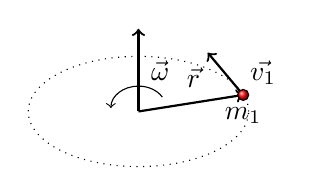
\begin{tikzpicture}[scale=.7]
  \draw[dotted] (1,.5) ellipse (2 and 1);
  \draw [<-,yscale=0.8] (.5,.7) arc (180:30:.5);

  \draw[->,thick] (1,.5)--(1,2); 
  \draw	(1,1.25)node[right=1pt]{$\vec{\omega}$};
     
\draw[->,thick] (1,.5) -- (2.9,.8);
\draw[<-,thick] (2.9,.8) +(130:1)--(2.9,.8)  ;
\draw (2,.7)node[above=1pt]{$\vec{r}$};
\draw	(2.8,1.2)node[right=1pt]{$\vec{v_1}$};
\draw (2.9,.8)node[below=1pt]{$m_1$};
\draw[shade,shading=ball,ball color=red] (2.9,.8) circle (.1);
 
\end{tikzpicture}
\end{boxleft}\begin{boxrightshaded}
\begin{align}
a_t		&=\alpha\cdot r\\
\vec{a_t}	&=\vec{\alpha} \times \vec{r}\\
\vec{\alpha}	&=\vec{r} \times \vec{a_t}\\
v		&=\omega\cdot r\\
\vec{v}		&=\vec{\omega}\times\vec{r}\\
\vec{\omega}	&=\vec{r} \times \vec{v}\\
s		&=\varphi\cdot r
\end{align}
\end{boxrightshaded}

\begin{boxleft}Winkelgeschwindigkeit,\\
Kreisfrequenz
\end{boxleft}\begin{boxrightshaded}
\begin{align}
\omega&=\frac{2\cdot\pi}{T}\\
&=2\cdot\pi\cdot n \\
&=2\cdot\pi\cdot f
\end{align}
\end{boxrightshaded}

\begin{boxleft}Bahngeschwindigkeit
\end{boxleft}\begin{boxrightshaded}
\begin{align}
v&=\frac{2\cdot \pi \cdot r}{T}\\
&=\omega\cdot r
\end{align}
\end{boxrightshaded}

\begin{boxleft}Radialbeschleunigung
\end{boxleft}\begin{boxrightshaded}
\begin{align}
a_r&=\frac{v^2}{r}\\
&=v\cdot\omega\\
&=\omega^2\cdot r
\end{align}
\end{boxrightshaded}

\begin{boxleft}Umdrehungen
\end{boxleft}\begin{boxrightshaded}
\begin{align}
N	&=\frac{\omega_0\cdot t}{2\cdot \pi}+\frac{1}{2}\cdot\frac{\alpha}{2\cdot \pi}\cdot t^2\\
	&=n_0\cdot t+\frac{\alpha}{4\cdot\pi}\cdot t^2
\end{align}
\end{boxrightshaded}

\section{Dynamik}
\subsection{Geradlinig(Translation)}
\begin{boxleft}Kraft
\end{boxleft}\begin{boxrightshaded}
\begin{align}
\vec{F}&=m\cdot \vec{a}\\
\vec{F}_{\text{Tr}}&=-m\cdot \vec{a}
\end{align}
\end{boxrightshaded}

\begin{boxleft}Impuls
\end{boxleft}\begin{boxrightshaded}
\begin{align}
\vec{p}&=m\cdot \vec{v}
\end{align}
\end{boxrightshaded}

\begin{boxleft}Kraftstoß
\end{boxleft}\begin{boxrightshaded}
\begin{align}
\vec{F}&=\frac{\diff \vec{p}}{\diff t}=m\cdot\frac{\diff \vec{v}}{\diff t}+\vec{v}\cdot\frac{\diff m}{\diff t}\\
\Delta\vec{p}&=\vec{p}_2-\vec{p}_1=\int_{\vec{p}_2}^{\vec{p}_1}\diff p=\int_0^{t}\vec{F}\diff t
\end{align}
\end{boxrightshaded}

\begin{boxleft}Arbeit
\end{boxleft}\begin{boxrightshaded}
\begin{align}
W&=-\int_{\vec{s}_1}^{\vec{s}_2}\vec{F_{\text{Tr}}}\circ\diff \vec{s}\\
&=\int_{\vec{v}_0}^{\vec{v}_1}m\vec{v}\circ\diff \vec{v}=\frac{1}{2}m\left(v_1^2-v_0^2\right) 
\end{align}
\end{boxrightshaded}

\begin{boxleft}kin. Energie
\end{boxleft}\begin{boxrightshaded}
\begin{align}
E_{\text{kin}}=\frac{1}{2}mv^2
\end{align}
\end{boxrightshaded}


\begin{boxleft}Hubarbeit
\end{boxleft}\begin{boxrightshaded}
\begin{align}
W_{\text{hub}}&=mgh
\end{align}
\end{boxrightshaded}

\begin{boxleft}Leistung
\end{boxleft}\begin{boxrightshaded}
\begin{align}
P=\vec{F}\circ\vec{v}=\frac{\diff W}{\diff t}=\dot{W}
\end{align}
\end{boxrightshaded}


\subsection{Drehbewegung(Rotation)}

\begin{boxleft}Massenträgheitsmoment
\end{boxleft}\begin{boxrightshaded}
\begin{align}
J=m\cdot r^2
\end{align}
\end{boxrightshaded}

\begin{boxleft}Drehimpuls
\end{boxleft}\begin{boxrightshaded}
\begin{align}
\vec{L}&=\vec{r}\times\vec{p} \\
&=J\cdot \vec{\omega}
\end{align}
\end{boxrightshaded}

\begin{boxleft}Drehmoment
\end{boxleft}\begin{boxrightshaded}
\begin{align}
\vec{M}&=\vec{r}\times\vec{F}=J\vec{\alpha}=\dot{\vec{L}}
\end{align}
\end{boxrightshaded}

\begin{boxleft}kinetische Energie
\end{boxleft}\begin{boxrightshaded}
\begin{align}
E_{kin}=\frac{1}{2}J\omega^2
\end{align}
\end{boxrightshaded}

\begin{boxleft}Arbeit
\end{boxleft}\begin{boxrightshaded}
\begin{align}
\Delta W	&=\int_{\varphi_0}^{\varphi_1}\vec{M}\circ\vec{e_\omega}\diff \varphi=\int_{\vec{\omega}_0}^{\vec{\omega}_1}J\vec{\omega}\diff\vec{\omega}\\
&=\frac{1}{2}J\left(\omega_1^2-\omega_0^2\right)
\end{align}
\end{boxrightshaded}

\begin{boxleft}Zentripedalkraft
\end{boxleft}\begin{boxrightshaded}
\begin{align}
F_{zp}&=-m\cdot\omega^2\cdot r\\
&=-m\cdot v^2\cdot \frac{\vec{e_r}}{r}
\end{align}
\end{boxrightshaded}

\subsection{Schiefe Ebene}

\begin{boxleft}Kräfte\\
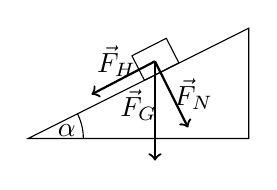
\begin{tikzpicture}[scale=.7]
  \draw (0,0) -- (4,0) -- (4,2)-- cycle;
  \draw[yshift=30,xshift=60,rotate=27] (0,0) -- (0,.5) -- (.7,.5) -- (.7,0) --cycle;
    
  \draw (1,0) arc (0:27:1);
  \draw (.7,0.15)node{$\alpha$};

  \draw[thick,->] (2.3,1.4)--(2.3,-.4);
  \draw[thick,->] (2.3,1.4)--(1.15,.8);
  \draw[thick,->] (2.3,1.4)--(2.9,.2);

  \draw (1.6,1.4)node{$\vec{F}_H$};
  \draw (3,0.8)node{$\vec{F}_N$};
  \draw (2,0.6)node{$\vec{F}_G$};
\end{tikzpicture}
\end{boxleft}\begin{boxrightshaded}
\begin{align}
\vec{F}_N&=\vec{F}_G\cos\alpha\\
\vec{F}_H&=\vec{F}_G\sin\alpha
\end{align}
\end{boxrightshaded}

\subsection{Reibung}

\begin{boxleft}Reibungskräfte
\end{boxleft}\begin{boxrightshaded}
\begin{align}
F_R=\mu\cdot F_N
\end{align}
\end{boxrightshaded}

\subsection{Feder}


\begin{boxleft}Hookesches Gesetz\\
$k$=$D$:Federkonstante,Richtgröße
\end{boxleft}\begin{boxrightshaded}
\begin{align}
F&=-kx=Dx\\
M&=D\varphi
\end{align}
\end{boxrightshaded}

\begin{boxleft}Spannungsenergie
\end{boxleft}\begin{boxrightshaded}
\begin{align}
W	&=\int_{x_\text{min}}^{x_\text{max}}F\diff x=\int_{x_\text{min}}^{x_\text{max}}kx\diff x\\
	&=\frac{1}{2}\cdot k\cdot \left(x_{\text{max}}^2-x_{\text{min}}^2\right)
\end{align}
\end{boxrightshaded}

\subsection{Elastischer Stoß}

\begin{boxleft}Energieerhaltung
\end{boxleft}\begin{boxrightshaded}
\begin{align}
\text{Energie vor den Stoß} &= \text{Energie nach den Stoß}\nonumber\\
\sum E_{\text{kin}}&=\sum E_{\text{kin}}'
\end{align}
\end{boxrightshaded}

\begin{boxleft}Impulserhaltung
\end{boxleft}\begin{boxrightshaded}
\begin{align}
\text{Impuls vor den Stoß} &= \text{Impuls nach den Stoß}\nonumber\\
\sum m\vec{v}&= \sum m\vec{v}'
\end{align}
\end{boxrightshaded}

\begin{boxleft}Zentraler, elastischer Stoß\\
(Energie und Impuls)
\end{boxleft}\begin{boxrightshaded}
\begin{align}
\frac{1}{2}m_1v_1^2+\frac{1}{2}m_2v_2^2&=\frac{1}{2}m_1v_1'^2+\frac{1}{2}m_2v_2'^2\\
m_1v_1+m_2v_2&=m_1v_1'+m_2v_2'
\end{align}
\end{boxrightshaded}

\begin{boxleft}Zentraler, elastischer Stoß\\
(Geschwindigkeit nach dem Stoß)
\end{boxleft}\begin{boxrightshaded}
\begin{align}
v_2'&=\frac{2m_1}{m_1+m_2}v_1+\frac{m_2-m_1}{m_1+m_2}v_2\\
v_1'&=\frac{2m_2}{m_1+m_2}v_2+\frac{m_1-m_2}{m_1+m_2}v_1
\end{align}
\end{boxrightshaded}

\subsection{Unelastischer Stoß}

\begin{boxleft}Energieerhaltung
\end{boxleft}\begin{boxrightshaded}
\begin{align}
\text{Energie vor den Stoß} &= \text{Energie nach den Stoß}+\text{Arbeit}\nonumber\\
\sum E_{\text{kin}}&=\sum E_{\text{kin}}'+\Delta W
\end{align}
\end{boxrightshaded}

\begin{boxleft}Impulserhaltung
\end{boxleft}\begin{boxrightshaded}
\begin{align}
\text{Impuls vor den Stoß} &= \text{Impuls nach den Stoß}\nonumber\\
\sum m\vec{v}&= \sum m\vec{v}'
\end{align}
\end{boxrightshaded}

\begin{boxleft}Total unelastischer Stoß\\
(Energie und Impuls)
\end{boxleft}\begin{boxrightshaded}
\begin{align}
\frac{1}{2}m_1v_1^2+\frac{1}{2}m_2v_2^2&=\frac{1}{2}\left(m_1+m_2\right)v'^2+\Delta W\\
m_1v_1+m_2v_2&=\left(m_1+m_2\right)v'
\end{align}
\end{boxrightshaded}

\begin{boxleft}Zentraler, elastischer Stoß\\
(Geschwindigkeit nach dem Stoß und Energieverlust)
\end{boxleft}\begin{boxrightshaded}
\begin{align}
v'		&=\frac{m_1v_1+m_2v2}{m_1+m_2}\\
\Delta W	&=\frac{m_1\cdot m_2}{2\left(m_1+m_2\right)}\left(v_1-v_2\right)^2
\end{align}
\end{boxrightshaded}

\subsection{Drehimpulse}

\begin{boxleft}Drehimpulserhaltungssatz
\end{boxleft}\begin{boxrightshaded}
\begin{align}
\text{Drehinpuls zur Zeit 1} &= \text{Drehimpuls zur Zeit 2}\\
\sum \vec{L}&=\sum \vec{L}'
\end{align}
\end{boxrightshaded}

\begin{boxleft}Kupplung Zweier Drehkörper\\
(Winkelgeschwindigkeit nach dem Kuppeln und Energieverlust)
\end{boxleft}\begin{boxrightshaded}
\begin{align}
\vec{\omega}'&=\frac{J_0\vec{\omega_0}+J_1\vec{\omega_1}}{J_1+J_2}\\
\Delta W&=\frac{J_0\cdot J_1}{2\left(J_0+J_1\right)}\left(\omega_0-\omega_1\right)^2
\end{align}
\end{boxrightshaded}


\subsection{Rotierendes Bezugssystem}

\begin{boxleft}Zentrifugalkraft
\end{boxleft}\begin{boxrightshaded}
\begin{align}
\vec{F}_Z&=F_r\cdot \vec{e}_r=-m\vec{\omega}\times\left(\vec{\omega}\times\vec{r}\right)=-m\vec{\omega}\times\vec{v}\\
  F_Z&=-m\frac{v^2}{r}=-m\omega^2 r
\end{align}
\end{boxrightshaded}

\begin{boxleft}Corioliskraft
\end{boxleft}\begin{boxrightshaded}
\begin{align}
\vec{F}_C&=-2m\vec{\omega}\times\vec{v}
\end{align}
\end{boxrightshaded}

\subsection{Schwerpunkt}

\begin{boxleft}Schwerpunkt mehrere Punktmassen
\end{boxleft}\begin{boxrightshaded}
\begin{align}
\vec{r}_{\text{Sp}}=\frac{\sum\vec{r}_i m_i}{\sum\ m_i}
\end{align}
\end{boxrightshaded}

\begin{boxleft}Allgemein Schwerpunkt
\end{boxleft}\begin{boxrightshaded}
\begin{align}
\vec{r}_{\text{Sp}}=\frac{\int \vec{r}\diff m}{\int \diff m}
\end{align}
\end{boxrightshaded}

\begin{boxleft}Schwerpunkt (Kartesische)
\end{boxleft}\begin{boxrightshaded}
\begin{align}
x_{\text{Sp}}&=\frac{\int_z\int_y\int_x x\rho \diff x \diff y \diff z }{\int_z\int_y\int_x \rho \diff x \diff y \diff z }\\
y_{\text{Sp}}&=\frac{\int_z\int_y\int_x y\rho \diff x \diff y \diff z }{\int_z\int_y\int_x \rho \diff x \diff y \diff z }\\
z_{\text{Sp}}&=\frac{\int_z\int_y\int_x z\rho \diff x \diff y \diff z }{\int_z\int_y\int_x \rho \diff x \diff y \diff z }
\end{align}
\end{boxrightshaded}

\begin{boxleft}Schwerpunkt (Zylinder)
\end{boxleft}\begin{boxrightshaded}
\begin{align}
r_{\text{Sp}}&=\frac{\int_z\int_\varphi\int_r r^2\rho \diff r \diff \varphi \diff z }{\int_z\int_\varphi\int_r r\rho \diff r \diff \varphi \diff z }\\
\varphi_{\text{Sp}}&=\frac{\int_z\int_\varphi\int_r \varphi r\rho \diff r \diff \varphi \diff z }{\int_z\int_\varphi\int_r r\rho \diff r \diff \varphi \diff z }\\
z_{\text{Sp}}&=\frac{\int_z\int_\varphi\int_r z r\rho \diff r \diff \varphi \diff z }{\int_z\int_\varphi\int_r r\rho \diff r \diff \varphi \diff z }\\
x&=r\cos{\varphi}\\
y&=r\sin{\varphi}\\
z&=z
\end{align}
\end{boxrightshaded}

\subsection{Trägheitsmoment}


\begin{boxleft}Allgemein
\end{boxleft}\begin{boxrightshaded}
\begin{align}
J&=\sum m_i r_i^2\\
J&=\int_m r^2 \diff m \\
J&=\int_z\int_\varphi\int_r r^3\rho \diff r \diff \varphi \diff z 
\end{align}
\end{boxrightshaded}

\begin{boxleft}Satz von Steiner\\(Parallel Verschiebung der Achse)
\end{boxleft}\begin{boxrightshaded}
\begin{align}
J_x&=mr^2+J_s
\end{align}
\end{boxrightshaded}

\begin{boxleft}Trägheitsmoment Kugel\\
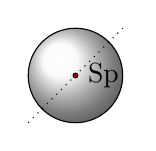
\begin{tikzpicture}[scale=.3]
  \draw[ball color=gray!5] (2,2) circle (2);
  \draw[fill=red] (2,2) circle (.1);
  \draw[dotted](0,0)--(4,4);
  \draw(2,2)node[right=1pt]{Sp};
\end{tikzpicture}\end{boxleft}\begin{boxrightshaded}
\begin{align}
J_\text{Sp}&=\frac{2}{5}mr^2
\end{align}
\end{boxrightshaded}

\begin{boxleft}Trägheitsmoment Zylinder\\
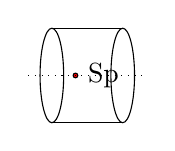
\begin{tikzpicture}[scale=.3]
  \draw (1,2) ellipse (.5 and 2);
  \draw (1,4) -- (4,4);
  \draw (1,0) -- (4,0);
  \draw (4,2) ellipse (.5 and 2);
  \draw[fill=red] (2,2) circle (.1);
  \draw[dotted](0,2)--(5,2);
  \draw(2,2)node[right=1pt]{Sp};
\end{tikzpicture}\end{boxleft}\begin{boxrightshaded}
\begin{align}
J_\text{Sp}&=\frac{1}{2}mr^2
\end{align}
\end{boxrightshaded}

\begin{boxleft}Trägheitsmoment Kreisring
\end{boxleft}\begin{boxrightshaded}
\begin{align}
J_\text{Sp}&=mr^2
\end{align}
\end{boxrightshaded}

\begin{boxleft}Trägheitsmoment Stab
\end{boxleft}\begin{boxrightshaded}
\begin{align}
J_\text{Sp}=\frac{1}{12}ml^2
\end{align}
\end{boxrightshaded}

\subsection{Elastizitätslehre}

\begin{boxleft}Spannung
\end{boxleft}\begin{boxrightshaded}
\begin{align}
\vec{\sigma}&=\frac{\vec{F}_n}{A}\\
\sigma&=E \varepsilon=E\frac{\Delta l}{l}
\end{align}
\end{boxrightshaded}

\begin{boxleft}Schubmodul
\end{boxleft}\begin{boxrightshaded}
\begin{align}
G&=\frac{\tau}{\varphi}
\end{align}
\end{boxrightshaded}

\begin{boxleft}Drillung
\end{boxleft}\begin{boxrightshaded}
\begin{align}
\psi&=\frac{\diff \varphi}{\diff l}=\frac{W_t}{G\cdot J_p}\tau=\frac{M_t}{G\cdot J_p}
\end{align}
\end{boxrightshaded}

\begin{boxleft}Polares Fläschenmoment
\end{boxleft}\begin{boxrightshaded}
\begin{align}
J_p&=\int r^2\diff A=\int_\varphi\int_r r^3\diff r \diff \varphi 
\end{align}
\end{boxrightshaded}

